\documentclass[a4paper,9pt]{extarticle}

%=========================================================
% PACKAGES
%=========================================================

\usepackage[
a4paper,
top=1.8cm,
bottom=1.5cm,
footskip=7mm,
left=1cm,
right=1cm,
headheight=14pt,
headsep=5mm
]{geometry}
\usepackage[T1]{fontenc}
\usepackage[utf8]{inputenc}
\usepackage[french]{babel}

\usepackage[sfdefault]{FiraSans}
\renewcommand{\familydefault}{\sfdefault}

\usepackage{multicol}
\setlength{\columnsep}{0.7cm}

\usepackage{amsmath,amssymb}

\usepackage{titlesec}
\usepackage{enumitem}

\usepackage{tcolorbox}
\tcbuselibrary{skins,breakable}

\usepackage{xcolor}

\usepackage{graphicx}
\usepackage{float}

\usepackage{tikz}

\usepackage{fancyhdr}
\usepackage[hidelinks]{hyperref}


%=========================================================
% PAGE SETTINGS
%=========================================================

\setlength{\parindent}{0pt}
\setlength{\parskip}{1.5pt}

\setlength{\abovedisplayskip}{4pt}
\setlength{\belowdisplayskip}{4pt}

\setlist[itemize]{
leftmargin=*,
itemsep=1pt,
topsep=1pt
}


%=========================================================
% COLORS
%=========================================================

\definecolor{Blue}{HTML}{E3F0FF}
\definecolor{Green}{HTML}{E3F7EA}
\definecolor{Pink}{HTML}{FFE5ED}
\definecolor{Orange}{HTML}{FFF0DC}
\definecolor{Purple}{HTML}{EEE7FF}
\definecolor{Yellow}{HTML}{FFFADB}


\definecolor{BlueTitle}{HTML}{285B8F}
\definecolor{GreenTitle}{HTML}{287052}
\definecolor{PinkTitle}{HTML}{A84063}
\definecolor{OrangeTitle}{HTML}{A96500}
\definecolor{PurpleTitle}{HTML}{6245A5}


%=========================================================
% HEADER
%=========================================================

\pagestyle{fancy}

\fancyhf{}

\fancyhead[L]{\small\textbf{Responsible Software}}
\fancyhead[C]{\small Fairness 2: Fairness in Machine Learning}
\fancyhead[R]{\small Week 08 --- 26/10-01/11/2026}

\fancyfoot[C]{\small\href{https://github.com/AlphaXT38G/notes_ba5}{github.com/AlphaXT38G/notes\_ba5}}
\fancyfoot[R]{\small \thepage}

\renewcommand{\headrulewidth}{0.4pt}



%=========================================================
% TITLES
%=========================================================

\titleformat{\section}
{\large\bfseries\color{BlueTitle}}
{}{0pt}{}

\titlespacing{\section}
{0pt}{6pt}{3pt}


% separator

\newcommand{\separator}{
\vspace{2pt}
\hrule
\vspace{3pt}
}


%=========================================================
% BOXES
%=========================================================

% Boxes are kept whole (unbreakable): inside multicols, a box split by tcolorbox
% leaves an empty column behind it.

% DEFINITION - blue
\newtcolorbox{definition}{
enhanced,
unbreakable,
colback=Blue,
colframe=BlueTitle,
boxrule=0.7pt,
arc=0mm,
title=\textbf{Definition},
fonttitle=\bfseries
}

% IMPORTANT - pink
\newtcolorbox{important}{
enhanced,
unbreakable,
colback=Pink,
colframe=PinkTitle,
boxrule=0.7pt,
arc=0mm,
title=\textbf{Key idea},
fonttitle=\bfseries
}

% FORMULAS - green
\newtcolorbox{formula}{
enhanced,
unbreakable,
colback=Green,
colframe=GreenTitle,
boxrule=0.7pt,
arc=0mm,
title=\textbf{Key formulas},
fonttitle=\bfseries
}

% WARNING - orange
\newtcolorbox{warning}{
enhanced,
unbreakable,
colback=Orange,
colframe=OrangeTitle,
boxrule=0.7pt,
arc=0mm,
title=\textbf{Warning},
fonttitle=\bfseries
}

% EXAMPLE - purple
\newtcolorbox{example}{
enhanced,
unbreakable,
colback=Purple,
colframe=PurpleTitle,
boxrule=0.7pt,
arc=0mm,
title=\textbf{Example},
fonttitle=\bfseries
}

% SUMMARY - orange
\newtcolorbox{summary}{
enhanced,
unbreakable,
colback=Yellow,
colframe=OrangeTitle,
boxrule=0.7pt,
arc=0mm,
title=\textbf{Summary},
fonttitle=\bfseries
}



% GOAT - brown: the idea told as simply as possible
\definecolor{Goat}{HTML}{F7EEDF}
\definecolor{GoatTitle}{HTML}{8A5A1F}
\newtcolorbox{goat}{
enhanced,
unbreakable,
colback=Goat,
colframe=GoatTitle,
boxrule=0.7pt,
arc=0mm,
title=\textbf{Explained to a goat},
fonttitle=\bfseries
}



%=========================================================
% FIGURE BOX
%=========================================================

\newtcolorbox{figurebox}{
enhanced,
colback=white,
colframe=gray,
boxrule=0.5pt,
arc=0mm,
center
}



%=========================================================
% DOCUMENT
%=========================================================

\begin{document}

%\footnotesize   --> To reduce the size of the text

\thispagestyle{fancy}



\begin{multicols}{2}


%=========================================================
\section{Mid-term Test}


\begin{summary}

\begin{itemize}

\item \textbf{2 November, 15:15}, 1h30 (+30 min special arrangements), assigned room and seat,
CAMIPRO on the table.

\item Paper, 12 pages; \textbf{one A4 sheet} (recto-verso, free format); no electronic device;
black or dark blue pen; SCIPER on top.

\item Single-choice + short answers: concise but full sentences, \textbf{1 point $\approx$ 1-2
sentences}; French allowed.

\end{itemize}

\end{summary}



%=========================================================
\section{Bias in Machine Learning}


\begin{definition}

\textbf{MACHINE LEARNING}: techniques that \textbf{infer patterns from data} that
\textbf{generalize to unseen data}. Algorithm = process (finds the parameters); model = result
(function + parameters). Training, then inference $y_u = f(x_u)$.

\end{definition}


\begin{formula}

\textbf{Supervised} (labels $y$): regression ($y$ continuous), classification ($y$ discrete).

\textbf{Unsupervised}: clustering, dimensionality reduction.

\end{formula}


\begin{important}

Sensitive to \textbf{data bias} (pre-existing, representation, measurement); labels often come
from \textbf{human annotation}.

\end{important}


\begin{center}

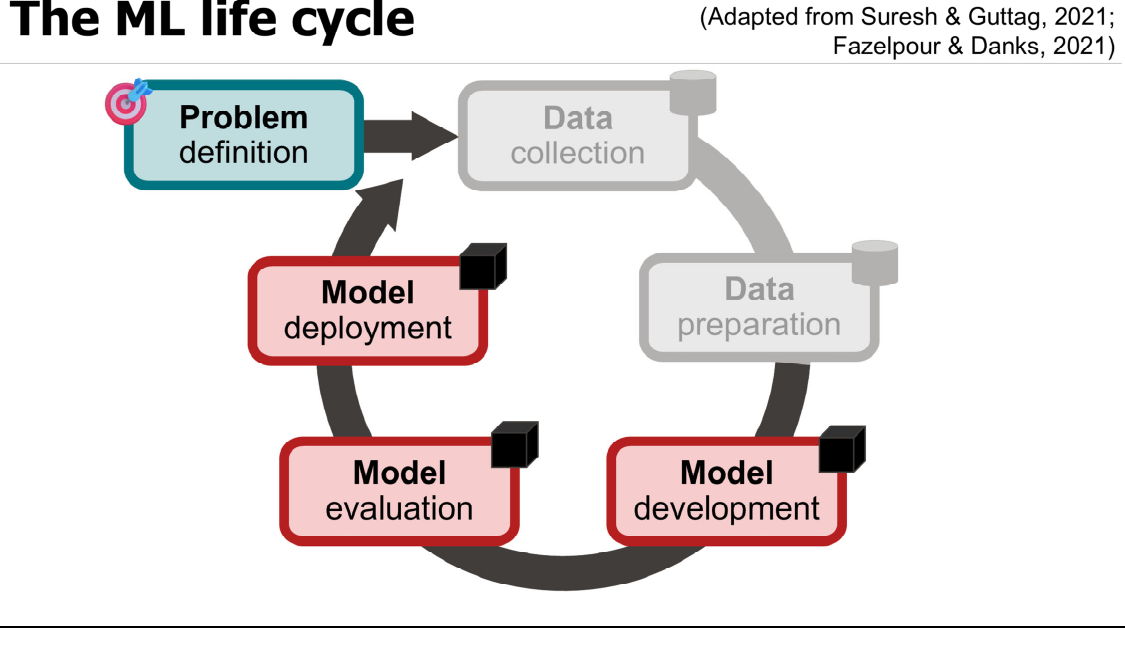
\includegraphics[
width=0.85\linewidth
]{../images/week08_02.png}

\end{center}


\begin{formula}

\textbf{Life cycle biases}

\begin{itemize}

\item \textbf{Optimization choices}: accuracy only $\Rightarrow$ unfairness.

\item \textbf{Aggregation bias}: different groups merged (Simpson's paradox).

\item \textbf{Evaluation bias}: benchmark $\neq$ served population (Gender Shades,
intersectional).

\item \textbf{Deployment bias}: used differently than intended.

\end{itemize}

\end{formula}


\begin{example}

Shoplifting detector tested on actors simulating thefts $\rightarrow$ \textbf{evaluation
bias}.

\end{example}


\begin{goat}

The machine learns a rule from examples. Bad examples, a rule mixing different goats, a test on
the wrong goats, or a use it was not made for: all give unfair answers.

\end{goat}



%=========================================================
\section{Group Fairness Criteria}


\begin{definition}

\textbf{FAIRNESS METRICS}: mathematical measures of \emph{certain} notions of fairness. Compare
the confusion matrices of \textbf{two groups}. (Criticisms: only equality, oversimplified,
blind optimization.)

\end{definition}


\begin{formula}

\textbf{Actual values} (ProPublica, \textbf{defendant}):
\[
\text{FNR} = \frac{FN}{TP+FN} \qquad \text{FPR} = \frac{FP}{TN+FP}
\]
\textbf{Predicted values} (NorthPointe, \textbf{decision-maker}):
\[
\text{FDR} = \frac{FP}{TP+FP} \qquad \text{FOR} = \frac{FN}{TN+FN}
\]
\textbf{Acceptance rate}:
\[
\frac{TP+FP}{TP+FP+FN+TN}
\]

\end{formula}


\begin{center}

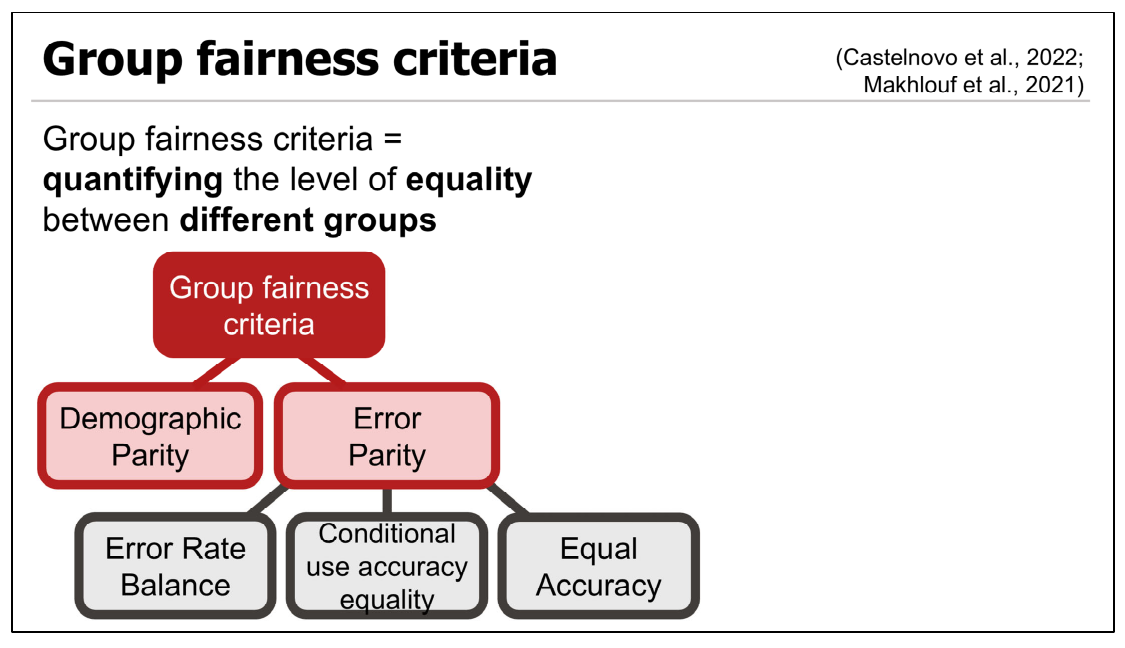
\includegraphics[
width=0.9\linewidth
]{../images/week08_06.png}

\end{center}


\begin{definition}

\textbf{ERROR PARITY} (outcome \emph{quality}): error rates independent of the group.

\begin{itemize}

\item \textbf{Error rate balance}: FPR, FNR (FNR only: equal opportunity).

\item \textbf{Conditional use accuracy equality}: PPV/FDR, NPV/FOR (PPV only: predictive
parity).

\item \textbf{Equal accuracy}.

\end{itemize}

\textbf{DEMOGRAPHIC PARITY} (outcome \emph{distribution}): equal acceptance rates
(statistical parity; disparate impact = ratio).

\end{definition}


\begin{warning}

\textbf{Impossibility}: different base rates + imperfect classifier $\Rightarrow$ the criteria
cannot all hold. Choosing one is a \textbf{moral dilemma}.

\end{warning}


\begin{example}

Fissures: plain $4/8$ vs. reinforced $3/9$ positive predictions $\rightarrow$
\textbf{demographic parity}, not satisfied. Every metric works for fairness if two groups are
compared.

\end{example}


\begin{goat}

Build the robot's mistake table for each colour of goat and compare: among the guilty, among the
accused, or how often each gets a ``yes''. You cannot equalise everything: choose.

\end{goat}



%=========================================================
\section{Fairness Returns}


\begin{formula}

\textbf{Beyond groups}: \textbf{intersectional} (combined groups; small samples),
\textbf{individual} (similar people, similar decisions; similarity measure), \textbf{causal}
(causal graphs; expert knowledge).

\textbf{Improving}: \textbf{pre-processing} (data: unawareness fails because of proxies,
reweighting, resampling), \textbf{in-processing} (training objectives), \textbf{post-processing}
(outputs; differential treatment).

\end{formula}


\begin{center}

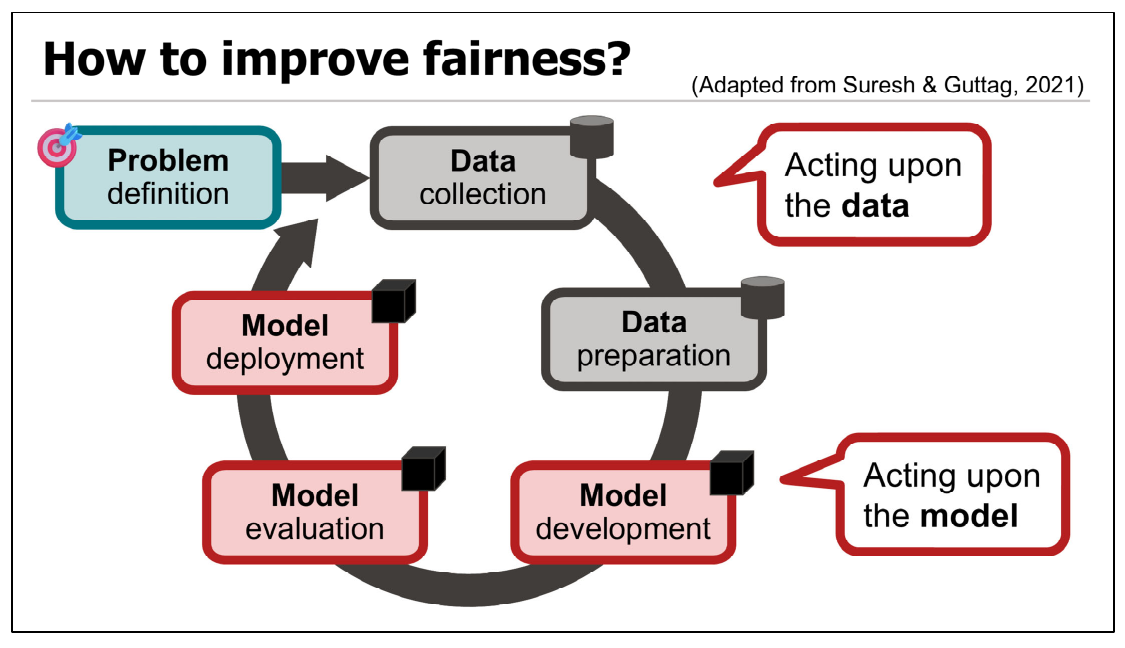
\includegraphics[
width=0.85\linewidth
]{../images/week08_08.png}

\end{center}


\begin{warning}

\textbf{Dilemmas}: leveling down; fairness vs. accuracy; fairness vs. privacy (sensitive
attributes needed).

\end{warning}


\begin{goat}

Fix the data before, the learning during or the answers after; each fix costs something.

\end{goat}



%=========================================================
\section{Strategy: Datasheets for Datasets}


\begin{formula}

\textbf{Datasheet} (Gebru 2021): motivation, composition, collection process, preprocessing,
uses, distribution, maintenance. Reveals issues; engineers spot ethical issues
\textbf{earlier and more often}.

\end{formula}


\begin{example}

\textbf{Face dataset}. Safety: no consent (authors, website), re-identification, offensive
content. Fairness: unclear population, no subgroup info, biased cropping. Model: unfit
population, different error rates.

Red flags: ``publicly available on the web'', \textbf{no ethical review}.

\end{example}


\textbf{Model cards}: the same for models (intended use, factors, metrics, intersectional
results, ethics).


\begin{goat}

A dataset needs an ID card; reading it shows the problems before your model learns them.

\end{goat}



%=========================================================
\section{Strategy: People Behind the Data}


\begin{formula}

IDEO AI Ethics Cards: \textbf{humanize} the data.

\begin{enumerate}

\item Find documentation, raw data.

\item Read the questionnaire, pick variables.

\item Pick participants, imagine their story.

\item Conclude on ethical impacts and risks.

\end{enumerate}

\end{formula}


\begin{center}

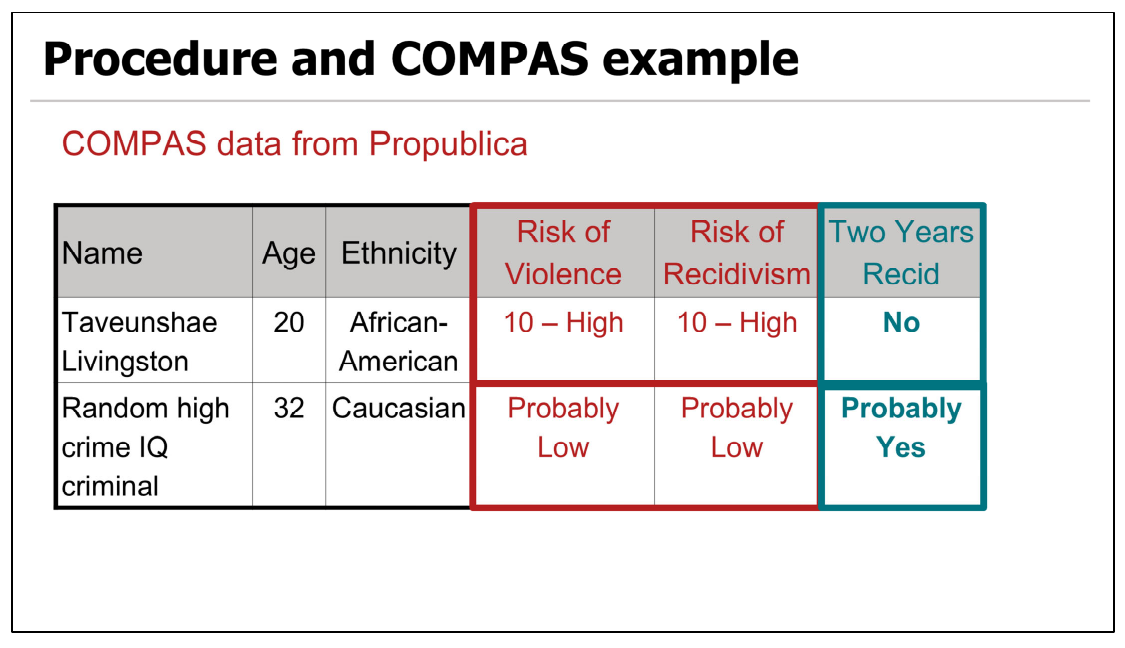
\includegraphics[
width=0.85\linewidth
]{../images/week08_09.png}

\end{center}


\begin{example}

\textbf{COMPAS}: a provocative young woman scores high risk but does not re-offend; a cunning
criminal answers ``safely'' and scores low. The questionnaire captures an environment people did
not choose (\textbf{pre-existing bias}) and oversimplifies lives (\textbf{measurement bias}).

\end{example}


\begin{goat}

Pick one row of the table and imagine the real goat behind it.

\end{goat}



%=========================================================
\section{Weekly Summary}


\begin{summary}

\begin{itemize}

\item ML flavours; aggregation, evaluation, deployment bias.

\item FNR / FPR (actual, defendant) vs. FDR / FOR (predicted, decision-maker).

\item Error parity (3 kinds) vs. demographic parity; impossibility.

\item Intersectional, individual, causal fairness; pre-, in-, post-processing.

\item Datasheets, model cards, people behind the data.

\end{itemize}

\end{summary}


\end{multicols}


\end{document}
